% ********** Chapter 2 **********
\chapter{Requirement}
\label{sec:Requirement}


\section{Programming Language}
\label{sec:Requirement:ProgrammingLanguage}

To make the application potable, \textbf{Java} is chosen as the programming language of Web Call SDK. The Java programming language is a popular high-level language which provides a portable feature and can be used on many different operating systems. For the introduction and more detail of Java please refer to \ref{sec:Solution:InvolvedTechnology:Java}.

\section{Simple}
\label{sec:Requirement:Simple}

The word ``Simple'' means, for community developers, the Web Call SDK should supplies a set of API that are easy to understand and convenient to use. The developers who use this API do not need much experience on java language and deep understanding of VoIP technology.

\section{Stability}
\label{sec:Requirement:Stability}

The application should be stable and has as less bugs as possible. The application should be designed for deploying on a server for long term use. The concurrent request users may more than one hundred. 

\section{Reusability}
\label{sec:Requirement:Reusability}

The code should be made as generic and reusable. The interface should not constrain on any specific network or service provider. It should follow a common accepted standard. Session Initiation Protocol (SIP) is a signalling protocol, which defined in RFC 3261 SIP: Session Initiation Protocol \cite{RFC3261}, widely used for multimedia communication sessions such as voice and video calls over the Internet. It should be used as the main signal protocol of Web Call SDK.

\section{Extendibility}
\label{sec:Requirement:Extendibility}
The application should be able to add new feature according to customer's requirement, e.g. add video call and instant message.

\section{Integration}
\label{sec:Requirement:Integration}

The Web Call SDK should supply a web service API that can be used by other applications. This interface should contain most of the functions of Web Call SDK. And can be easily used on Web 2.0\footnote{``Web 2.0'' refers to a perceived second generation of web development and design, that facilitates communication, secure information sharing, interoperability, and collaboration on the World Wide Web.\cite{Web2dot0} See also: \href{http://www.oreillynet.com/pub/a/oreilly/tim/news/2005/09/30/what-is-web-20.html}{What Is Web 2.0}\cite{WhatIsWeb2dot0}} mashup\footnote{Mashup is a Web application that combines data or functionality from two or more sources into a single integrated application.}.






Based on IMS/SIP network technology, Web Call SDK integrated call functions into Web containers. This presents a simple way to implement the communication convergence of Web, IMS/SIP network, and CS networks. It does not require the installation of the plug-in clients on the browser or other special client software as most VoIP services.

Compare to other customer-oriented VoIP products, Web Call SDK offers solutions for developers. It integrated the SIP call function into Web container as Java EE components, providing the example of the convergences between SIP/IMS and the Internet Web technology.

\begin{figure}
\centering
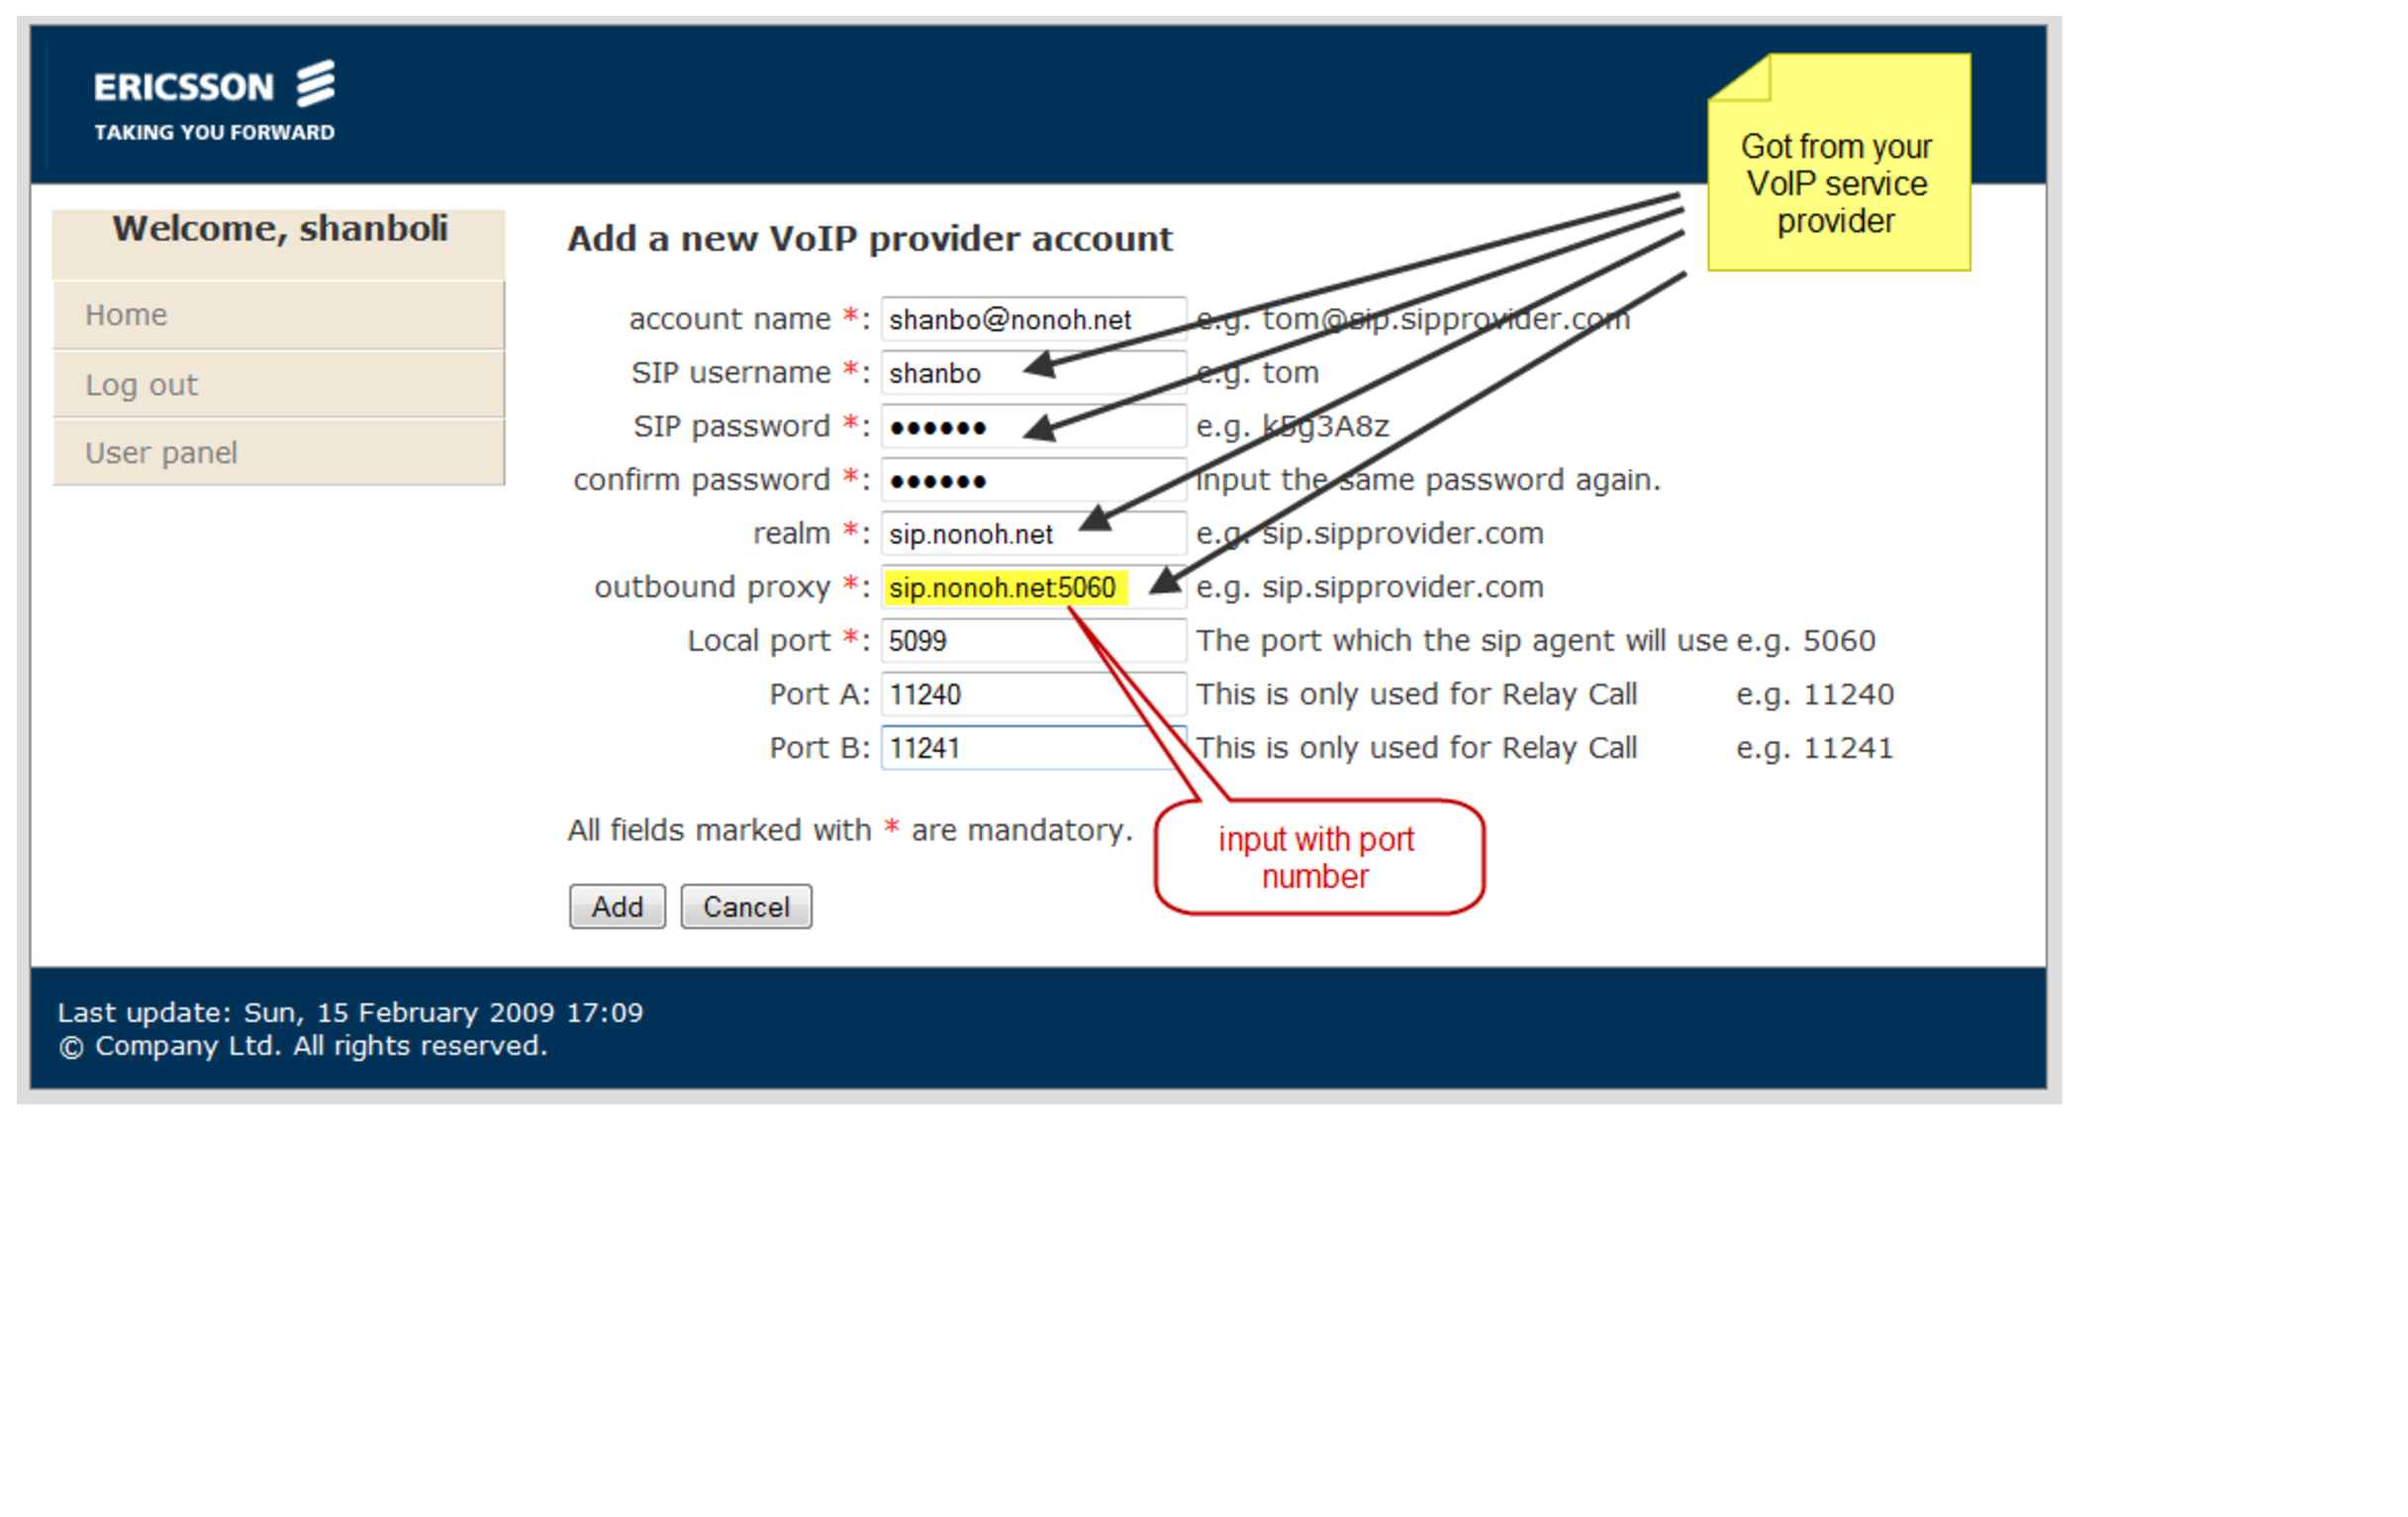
\epsfig{file=chap01/test_picture, height=4in}
\caption{A sample black and white graphic (.eps format).}
\end{figure}

... some text\index{text} ...

Some reference~
abc\cite{RFC3261}\\
def\cite{RFC3725}

%Some symbols: DMC\label{sym:DMC}, LZ77\label{sym:LZ77}, LZ78\label{sym:LZ78}.

% ********** End of chapter **********
